%
% Definitiestudie
%

\chapter{Definitiestudie}

Voorafgaand aan de start van het spel is er een inschrijvingsperiode. (Uitbreiding: Spelers kunnen zich registeren met behulp van hun eID.) Spelers die zich registeren voor de start van het spel verkrijgen 100.000 euro virtuele cash.

Het spel start op een vastgesteld moment: op 1 maart 2010 om 8u 's morgens, Central European Time. Gebruikers die na de start van het spel registreren krijgen een ander startbudget. Maximaal verkrijgen de spelers een startbudget van 100.000 euro. Is de re\"ele beurs sinds de start van het spel negatief ge\"evolueerd, dan wordt het startbudget ook in verhouding evenveel verlaagd.

Van zodra gebruikers geregistreerd zijn, hebben de gebruikers toegang tot hun portfolio en kunnen daar effecten aan worden toegevoegd.

De gebruiker kan effecten aankopen en verkopen van onderstaande types:
\begin{itemize_compact}
	\item{aandelen op de Continumarkt van Brussel}
	\item{aandelen op de Eurolist van Parijs}
	\item{aandelen op de Lokaal van Amsterdam}
	\item{trackers op Euronext Amsterdam}
\end{itemize_compact}

Tijdens het verloop van het spel worden er op gezette tijden (per dag, per week en per maand) klassementen opgemaakt met daarin het relatief rendement dat de spelers konden neerzetten. Op basis van deze tussenklassementen worden er ook punten toegekend, waarmee ook een apart puntenklassement wordt opgemaakt. Dit puntenklassement geeft een eerlijkere kijk op de prestaties van de speler, en zorgt ervoor dat niet enkel het uiteindelijke rendement tussen de start- en einddatum van belang is, maar ook de continue goede prestaties tijdens de duur van het spel.

Het spel eindigt op 31 mei 2010, waarna een eindklassement wordt opgemaakt. De koersen op de website worden niet meer geüpdatet, en er kunnen ook geen transacties meer gedaan worden. Gebruikers kunnen wel nog steeds authenticeren op de website om statistieken van hun spelverloop te raadplegen.


\section{Website}

\begin{figure}[h!]
	\centering
		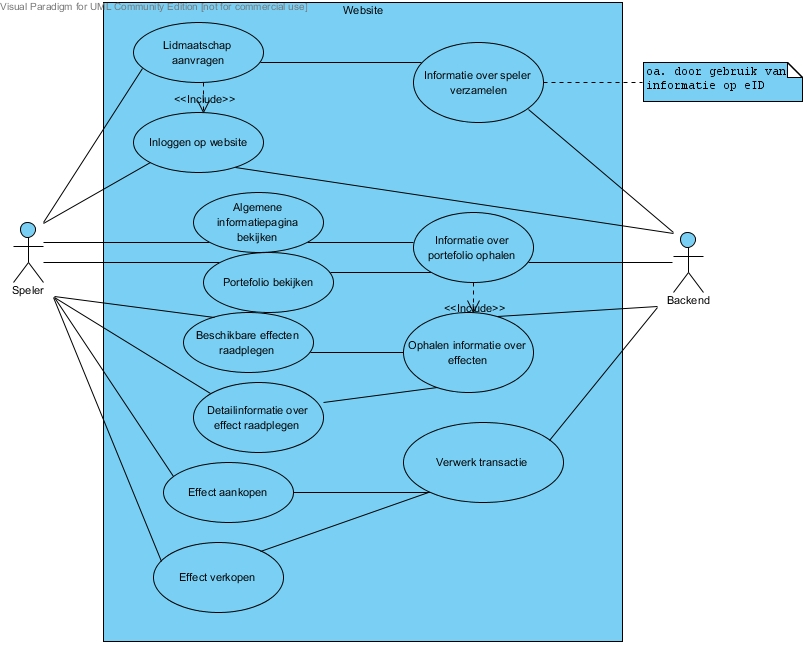
\includegraphics[width=0.5\textwidth]{images/analyse/ucd_website}
	\caption{Use-case diagram van de website.}
\end{figure}

\subsection{Uitwerking use cases}

\subsubsection{Lidmaatschap aanvragen}
\begin{compact}
\paragraph{Beschrijving}Een persoon kan zich inschrijven voor een lidmaatschap. Dit lidmaatschap is een vereiste om de interactieve delen van de website te kunnen beleven. Deze procedure bestaat uit een aantal velden die naar waarheid in te vullen zijn en een aantal velden waar men een waarde voor kan kiezen.
\paragraph{Primaire actoren}Een persoon die de interactieve delen van de website wil gebruiken
\paragraph{Doel}De speler verkrijgt een lidmaatschap. Via dit lidmaatschap kunnen we een persoon (een speler) koppelen aan zijn portfolio.
\paragraph{Precondities}De speler bezitte een geldig email adres, een eID lezer en hij was nog niet in bezit van een lidmaatschap (een persoon bezit een lidmaatschap als hij de combinatie gebruikersnaam en wachtwoord kent of over een eID bezit waar een lidmaatschap aan gekoppeld is). \small{Lidmaatschap aanvragen is pas mogelijk vanaf 1 maart 2010, 8u, Central European Time.}
\paragraph{Postcondities}In de database zit een nieuw record waarmee we de speler kunnen authenticeren en waaraan zijn instellingen en portfolio gekoppeld worden.
\paragraph{Triggers}Een persoon zit op de inleidende website en kiest daar voor de optie ``Registreren''.
\paragraph{Notities}De velden die de gebruiker op de afzonderlijke registratie pagina dient in te vullen zijn terug te vinden in het database schema van de gebruikers. Alle velden zijn verplicht.
\paragraph{Business rules}Het registreren (en dus onrechtstreeks het spelen van het beursspel) moet aangemoedigd worden vanuit de gastsite.
\paragraph{Prioriteit}Gemiddeld
\paragraph{Complexiteit}Laag
\paragraph{Successcenario}
\begin{enumerate_compact}
 \item Speler bezoekt de website
 \item Speler maakt de keuze dat hij mee wil spelen
 \item Speler geeft aan te willen registreren
 \item Speler vult alle vereiste velden in
 \item Speler vult eventueel enkele optionele velden in
 \item Speler bevestig zijn registratie
 \item \label{def:lidmaatschap:bevestiging} Speler krijgt een bevestiging van zijn registratie
\end{enumerate_compact}
\paragraph{Alternatieve scenario's}
Alternatief voor \ref{def:lidmaatschap:bevestiging}:
\begin{itemize_compact}
 \item Speler is een vereist veld vergeten en krijgt de mogelijkheid om dit aan te passen
 \item Speler heeft een ongeschikte of foutieve invoer gedaan voor een veld en krijgt de mogelijkheid om dit aan te passen
\end{itemize_compact}
\end{compact}
 
\subsubsection{Het bekijken van de gastsite}
\begin{compact}
\paragraph{Beschrijving}De website zal uit drie delen bestaan. Een deel bestaat uit een of meerdere pagina's. Een deel zal enkel zichtbaar zijn voor niet geauthenticeerde gebruikers of bezoekers zonder lidmaatschap. Een ander deel zal zichtbaar zijn voor zowel niet geauthenticeerde bezoekers als geauthenticeerde bezoekers. Geauthenticeerde bezoekers hebben dan ook nog toegang tot een enkel voor hen zichtbare derde deel. Het is in dat deel dat de interactieve site zich bevindt.
\paragraph{Primaire actoren} Bezoekers zonder lidmaatschap die er wel een willen aanvragen, bezoekers zonder lidmaatschap die enkel op zoek zijn naar informatie over het spel en bezoekers met lidmaatschap die zich willen authenticeren voor toegang tot het voor hen zichtbare deel.
\paragraph{Doel} Bezoekers snel laten inloggen, bezoekers informeren over het spel, bezoekers doorheen de registratieprocedure leiden.
\paragraph{Precondities} De gastsite heeft dezelfde precondities als de overige delen van de website. De surfer was voorzien van een breedband internetverbinding, een desktop of draagbare computer met daarop een gangbaar en recent besturingssysteem en bijhorende standaard compatibele internetbrowser.
\paragraph{Postcondities} De gebruiker was ingelogd, geregistreerd of was voldoende ge\"informeerd over het spel.
\paragraph{Triggers} De surfer bezoekt de website door het ingeven van het webadres, het aanklikken van een favoriet in zijn internetbrowser of na het klikken op een webverwijzing op een andere internetwebsite.
\paragraph{Notities} Het gastgedeelte zal op elke pagina een module bevatten waarmee bezoekers met lidmaatschap zich snel kunnen authenticeren.\small{Om de surfer te informeren over het spel zullen verschillende pagina's voorzien worden. Op die pagina's zijn visuele hulpmiddelen voorzien zoals afbeeldingen waarop te zien is hoe bepaalde spelprocedures verlopen en eventueel ook ondersteunde filmen.}
\paragraph{Business rules}Het is op dit gedeelte van de site dat de surfer en potenti\"ele speler overtuigd moet worden om actief mee te spelen.
\paragraph{Prioriteit}Laag
\paragraph{Complexiteit}Laag
\paragraph{Successcenario}
\begin{enumerate_compact}
 \item Speler bezoekt de website
 \item Speler navigeert naar de juiste pagina
 \item Speler is voldoende ge\"informeerd
\end{enumerate_compact}
\end{compact}

\todo{De beschrijving van deze use case is gewoon een kopie van de vorige?? -Dieter}
\subsubsection{Inloggen}
\begin{compact}
\paragraph{Beschrijving} De website zal uit drie delen bestaan. Een deel bestaat uit een of meerdere pagina's. Een deel zal enkel zichtbaar zijn voor niet geauthenticeerde gebruikers of bezoekers zonder lidmaatschap. Een ander deel zal zichtbaar zijn voor zowel niet geauthenticeerde bezoekers als geauthenticeerde bezoekers. Geauthenticeerde bezoekers hebben dan ook nog toegang tot een enkel voor hen zichtbare derde deel. Het is in dat deel dat de interactieve site zich bevindt. Dat deel is enkel toegankelijk voor geauthenticeerde bezoekers.
\paragraph{Actoren} Bezoekers met lidmaatschap die toegang willen tot het interactieve deel van de website.
\paragraph{Doel} Een bezoeker koppelen aan zijn lidmaatschap en dus onrechtstreeks aan zijn portfolio, puntentotaal en instellingen.
\paragraph{Precondities} De bezoeker bezit reeds een lidmaatschap en beschikt over voldoende informatie en hulpmiddelen om aan te kunnen tonen dat dit lidmaatschap van hem of haar is.
\paragraph{Postcondities} De gebruiker is geauthenticeerd.
\paragraph{Triggers} De gebruiker vult zijn gebruikersnaam en wachtwoord in of verbind zijn eID met de applicatie. Dit gebeurt vanaf de gastpagina.
\paragraph{Notities} Het kan zijn dat de gebruiker niet moet inloggen omdat dit reeds voorheen gebeurd is en een bepaald mechanisme met een cookie de authenticatie reeds verzocht heeft. Dit laatste gebeurt dan onzichtbaar voor de gebruiker.
\paragraph{Prioriteit}Hoog
\paragraph{Complexiteit}Hoog
\paragraph{Successcenario}
\begin{enumerate_compact}
 \item Speler bezoekt de website
 \item Speler geeft voldoende gegevens waarmee hij zich kan authenticeren
 \item \label{def:inloggen:bevestiging} Speler krijgt een bevestiging en wordt doorgestuurd naar het interactieve deel van de website
\end{enumerate_compact}
\paragraph{Alternatieve scenario's}
Alternatief voor \ref{def:inloggen:bevestiging}:
\begin{enumerate_compact}
 \item Speler heeft een ongeschikte of foutieve invoer gedaan voor een veld en krijgt de mogelijkheid om dit aan te passen
\end{enumerate_compact}
\end{compact}

\subsubsection{De gebruiker bekijkt zijn eigen Portfolio}
\begin{compact}
\paragraph{Beschrijving} De gebruiker ziet een webpagina met daarop de effecten die deze momenteel in bezit heeft, de historische aankoopprijs per stuk, de historische aankoopprijs in totaal, de huidige koers, het rendement en het verschil op de waarde sinds de aankoop van het effect.
\paragraph{Actoren} De speler bekijkt het portfolio. De huidige waarde hangt af van de re\"ele beursevolutie (de scrapers volgen deze evolutie).
\paragraph{Doel} De gebruiker ziet zijn portfolio en de gegevens die interessant zijn om erbij te zien.
\paragraph{Precondities} De gebruiker is ingelogd.
\paragraph{Triggers} De gebruiker kiest in het linkermenu de optie ``Portfolio''.
\paragraph{Prioriteit}Hoog
\paragraph{Complexiteit}Laag
\paragraph{Successcenario}
\begin{enumerate_compact}
 \item De gebruiker geeft aan zijn portfolio te willen bekijken
 \item De gebruiker definieert een filtering of een combinatie van filters
 \item Een overzicht van de speler zijn huidige portfolio wordt getoond
\end{enumerate_compact}
\end{compact}

\todo{In deze use case staan al die verschillende orders beschreven. Maar die staan al uitgewerkt in ``Module geavanceerde orders''! Het lijkt me best om hier gewoon een opsomming te geven van de mogelijkheden en te refereren naar dat ander hoofdstuk.}
\subsubsection{Effecten aankopen}
\begin{compact}

\paragraph{Overzicht}Een gebruiker kan zijn portfolio invullen of aanvullen door effecten bij te kopen. De speler kan effecten bijkopen van een effect die hij/zei reeds bezit of een nieuwe reeks aankopen. Een effect kan nooit rechtstreeks aangekocht worden, dit gebeurt met een tussenstap. Deze tussenstap noemen we het plaatsen van een order. Een order bestaat er in twee types; een aankooporder of een verkooporder. Een order heeft een voorwaarde, type, aantal, eigenaar en effect. Orders worden periodiek (elke minuut) bekeken. Als aan de voorwaarde voldaan wordt, dan wordt het order omgezet in een effectieve aankoop of verkoop. Dan pas worden de effecten toegevoegd of verwijderd van het spelers portfolio. Het kan dus zijn dat een geplaatst order pas in de verre toekomst uitgevoerd wordt of in zijn geheel niet uitgevoerd wordt. De voorwaarden die op een order ingezet kunnen worden houden we in een eerste fase beperkt. Maar deze kunnen later aangevuld worden met geavanceerde orders, zoals ook te zien is bij de huidige gespecialiseerde brokers. We beginnen met drie typen van orders:

\begin{itemize_compact}
 \item Voer onmiddellijk uit, ongeacht de huidige koers.
 \item Koerslimiet: Voer een aankoop order uit als de prijs lager is dan de ingestelde limietwaarde
 \item Koerslimiet: Voer een verkoop order uit als de prijs hoger is dan de ingestelde limietwaarde
\end{itemize_compact}

Mogelijke geavanceerde orders die we in een verdere fase zouden kunnen invoeren zijn de volgende:
\begin{itemize}
	\item Trailling-stop: Bij een verkoop order wordt de trigger waarde ingesteld op een vast aantal beurspunten onder de hoogste koers. Als de hoogste koers dus verhoogd in waarde, dan verhoogd ook de trigger waarde evenveel punten. Deze tactiek gebruikt de speler als die verwacht dat de waarde van het effect nog wel een tijdje zal toenemen, maar hij toch zijn winst wil veiligstellen. Hetzelfde kan ook ingesteld worden bij een aankooporder. Als de speler namelijk verwacht dat de waarde van een effect nog een tijdje zal blijven dalen, en de speler laag wil inkopen.
  \item Bracket-limiet: De speler kan met dit type order de maximale fluctuaties van zijn effect beperken. Hij stelt twee waardes in waar het order omgezet zal worden in een effectieve handeling. Dit is een waarde boven de huidige koers en een waarde onder de huidige koers. Zo beperkt de speler dus zijn maximaal verlies, maar ook zijn maximale winst. De waardes tussen de hoogste en laagste limietwaarde is de bandbreedte waar het effect kan tussen schommelen terwijl het in de portefeuille blijft van de speler.
  \item Stop loss order: Een order wordt omgezet in een effectieve handeling ongeacht de limietwaarde. Het order wordt hierdoor sneller uitgevoerd, maar er is geen minimumprijs (maximumprijs) gegarandeerd.
\end{itemize}
\paragraph{Prioriteit}Laag
\paragraph{Complexiteit}Laag
\paragraph{Successcenario}
\begin{enumerate_compact}
 \item Speler geeft vanuit een overzichtspagina of detailpagina aan dat hij een order wil plaatsen op een effect
 \item Speler geeft de order specificaties op (aantal effecten, type, limieten, )
 \item Speler bevestigd zijn order
 \item \label{def:aankopen:bevestiging} Speler krijgt een bevestiging van zijn order
\end{enumerate_compact}
\paragraph{Alternatieve scenario's}
Alternatief voor \ref{def:aankopen:bevestiging}:
\begin{enumerate_compact}
 \item Speler heeft een ongeschikte of foutieve invoer gedaan voor een veld en krijgt de mogelijkheid om dit aan te passen
\end{enumerate_compact}
\end{compact}

\subsubsection{Effecten verkopen}
\begin{compact}
Een effect verkopen verloopt op dezelfde manier als een effect aankopen. Er wordt ook een order aangemaakt voor een aantal effecten. Resulteert de voorwaarde van het order positief, dan worden zoveel effecten verkocht. Als een gebruiker geen effecten meer overhoudt van een bepaald symbool, dan wordt dit uit het portfolio gehaald.
\paragraph{Actoren} De speler plaatst een order
\paragraph{Doel} Een order plaatsen welke tot doel heeft omgezet te worden in een effectief order. Dit wordt bepaald door de voorwaarde die ge\"evalueerd wordt ten op zichte van de huidige beursevolutie. Het onrechtstreekse doel is het uitbreiden van het virtueel portfolio van de speler.
\paragraph{Precondities} De gebruiker zijn cash positie moet voldoen om het order te plaatsen en uit te voeren.
\paragraph{Postcondities} Een order is geplaatst en kan later uitgevoerd worden, mislukken of verlopen.
\paragraph{Triggers} De aankooppagina wordt getoond door het activeren van een optie op een effectenpagina.
\paragraph{Prioriteit}Laag
\paragraph{Complexiteit}Laag
\paragraph{Successcenario}
\begin{enumerate_compact}
 \item Speler geeft vanuit een overzichtspagina of detailpagina aan dat hij een order wil plaatsen op een effect
 \item Speler geeft de order specificaties op (aantal effecten, limieten, )
 \item Speler bevestigd zijn order
 \item \label{def:verkopen:bevestiging} Speler krijgt een bevestiging van zijn order
\end{enumerate_compact}
\paragraph{Alternatieve scenario's}
Alternatief voor \ref{def:verkopen:bevestiging}:
\begin{enumerate_compact}
 \item Speler heeft een ongeschikte of foutieve invoer gedaan voor een veld en krijgt de mogelijkheid om dit aan te passen
\end{enumerate_compact}
\end{compact}

\subsubsection{Overzicht opvragen van de effecten die je in het spel actief kan verhandelen}
\begin{compact}
\paragraph{Beschrijving} Een effect op de beurs kan ofwel opgenomen worden door onze scrapers of buiten bereik liggen van onze scrapers.
Als deze binnen het bereik van een of meerdere scrapers valt, dan worden er gegevens van bijgehouden in onze dataopslag. Een effect kan dan nog onderverdeeld worden onder effecten die onzichtbaar zijn op de site, effecten die geschorst zijn en dus niet actief verhandeld kunnen worden en actief te verhandelen effecten. Bij het overzicht worden de gescrapete actieve of geschorste effecten getoond. Hierop kunnen dan filters geplaatst worden om de lijst in te korten.
\paragraph{Doel} Een effect kunnen vinden waarvan je de detailpagina wil bekijken. Met het onrechtstreekse doel op het geschikte effect een order te plaatsen. Een detail pagina vind je door in het overzicht een aandeel aan te klikken.
\paragraph{Postcondities} De speler ziet een pagina met daarin een lijst van effecten die voldoen aan zijn ingestelde of geselecteerde filter
\paragraph{Triggers} Via het menu vraagt de speler de overzichtspagina op
\paragraph{Notities} Er kan een combinatie van volgende filters ingesteld worden op de site:

\begin{itemize_compact}
	\item Type
	\item Beurs
	\item Index
	\item Deelstring van de naam
	\item Effecten met een vlagje (favoriete aandelen)
	\item Per prijs ($<$ $>$ = $\leq$ $\geq$)
	\item Per volume
	\item Per aantal persoonlijke verhandelingen op het effect
	\item Per aantal verhandelingen van medespelers in het spel op het effect ((on-)populaire effecten)
\end{itemize_compact}

\paragraph{Notities}In het overzicht zijn naast de link naar de detailpagina ook knoppen voorzien om rechtstreeks een aankoop of verkoop order te plaatsen op een bepaald effect.
\paragraph{Business rules}Een aantal combinaties van filters moeten reeds vooraf ingesteld worden door de beheerders en gemakkelijk te selecteren zijn vanuit het menu.
\paragraph{Prioriteit}Laag
\paragraph{Complexiteit}Laag
\paragraph{Successcenario}
\begin{enumerate_compact}
 \item De gebruiker geeft aan een overzicht te willen bekijken
 \item De gebruiker definieert een filtering of een combinatie van filters
 \item De gebruiker bevestigd zijn filter en krijgt een overzicht van de resultaten die daaraan voldoen
\end{enumerate_compact}
\end{compact}

\subsubsection{Een klassement opvragen}
\begin{compact}

\paragraph{Beschrijving} Er bestaat een overzichtspagina waar gastgebruikers en geauthenticeerde spelers een overzicht kunnen zien van:
\begin{itemize_compact}
	\item De top 10 effecten die het meest aangekocht zijn op een specifiek tijdsinterval
	\item De top 10 effecten die het meest verkocht zijn op een specifiek tijdsinterval
	\item De top 20 spelers met het hoogst behaalde rendement tijdens het geselecteerde tijdsinterval
\end{itemize_compact}
Het tijdsinterval kan de speler bepalen door een dubbele slider te verslepen. Deze slider heeft een beginpunt en een eindpunt. De periode wordt bepaald door deze twee punten en dus de grote van de periode door het verschil van het eindpunt en het beginpunt.
\paragraph{Triggers} De surfer selecteert het overzichtsscherm in het menu op de linkerzijde van het scherm.
\paragraph{Notities} De resultaten worden getoond in tabellen die via een synchrome AJAX request opgehaald worden na het verplaatsen van een van beide punten van de slider.
\paragraph{Prioriteit}Laag
\paragraph{Complexiteit}Laag
\end{compact}

\subsubsection{Een detail fiche bekijken}
\begin{compact}
\paragraph{Beschrijving} De detail fiche heeft tot doel de speler of bezoeker zoveel mogelijk informatie te verschaffen over de huidige en historische stand van een effect.
\paragraph{Doel} De speler of bezoeker genoeg informatie verschaffen zodat hij op basis daarvan kan bepalen of het interessant zou zijn een order te plaatsen op het aandeel. Eventueel kan de speler het effect een vlagje geven (favoriet aandeel). Zodoende vindt hij/zij het dan later vlugger terug door het zetten van de geschikte filter.
\paragraph{Triggers} De detailpagina kan de speler bereiken door in zijn portfolio op een effect te klikken. Spelers of gastgebruikers vinden de pagina door de weblink te gebruiken op een al dan niet gefilterde overzichtspagina. Eventueel kan ook de directe link van de detail pagina gebruikt worden. Die directe link kan direct bezocht worden, opgevraagd worden uit de favorieten van de browser of via een weblink op een andere webpagina aangeboden worden.
\paragraph{Notities} Op deze pagina wordt het mogelijk gemaakt een favorietenvlag te zetten of weg te halen, naar de aankooppagina te gaan van dit effect of naar de verkooppagina te gaan van dit effect.
\paragraph{Prioriteit}Laag
\paragraph{Complexiteit}Laag
\paragraph{Successcenario}
\begin{enumerate_compact}
 \item Gebruiker begin bij scenario ``Overzicht opvragen van de effecten die je in het spel actief kan verhandelen'' of bij "De gebruiker bekijkt zijn eigen Portfolio"
 \item In het overzicht geeft de gebruiker aan de details van een effect te willen bekijken
 \item Alle beschikbare informatie van een effect wordt getoond samen met een interactieve grafiek
\end{enumerate_compact}
\end{compact}

\subsubsection{Gebruiker bekijkt zijn transactiegeschiedenis}
\begin{compact}
\paragraph{Beschrijving} Een gebruiker bekijkt zijn transactiegeschiedenis op een daarvoor ingerichte pagina. De gebeurtenissen op die pagina zijn te filteren op:
\begin{itemize_compact}
	\item Type
	\item Transacties die winst opleveren volgens de huidige beursevolutie
	\item Het tijdstip
	\item Het effect
	\item Het aantal
	\item Het verschil in waarde sinds de aankoop en het huidige moment
\end{itemize_compact}
\paragraph{Prioriteit}Laag
\paragraph{Complexiteit}Laag
\paragraph{Successcenario}
\begin{enumerate_compact}
 \item Gebruiker geeft aan zijn transactiegeschiedenis te willen bekijken
 \item Gebruiker krijgt een overzicht van zijn transactiegeschiedenis te zien
\end{enumerate_compact}
\end{compact}

\subsubsection{Gebruiker bekijkt zijn algemeen overzicht}
\begin{compact}
\paragraph{Beschrijving} Een gebruiker bekijkt zijn algemeen overzichtspagina en vindt hierop zeker volgende waardes opgesomd:
\begin{itemize_compact}
	\item De huidige waarde dat zijn portfolio en cashpositie samen vertegenwoordigen
	\item Cashpositie
	\item Huidig rendement
	\item Een grafiek met daarop volgende lijnen geplot in functie van de tijd:
  \begin{itemize_compact}
  	\item  Overzicht van hun rendement
    \item Overzicht van het gemiddelde rendement
    \item Overzicht van het rendement van de speler met het op dat moment hoogste rendement
  \end{itemize_compact}
  \item Een algemeen klassement en de positie van de speler daarin
  \item Een klassement van de huidige periode en de positie van de speler daarin
\end{itemize_compact}
\paragraph{Prioriteit}Laag
\paragraph{Complexiteit}Laag
\paragraph{Successcenario}
\paragraph{Successcenario}
\begin{enumerate_compact}
 \item Gebruiker krijgt zijn algemeen overzicht te zien na inloggen of geeft aan zijn transactiegeschiedenis te willen bekijken
 \item Gebruiker krijgt een algemeen overzicht te zien
\end{enumerate_compact}
\end{compact}


\section{Desktopapplicatie}

\subsection{Uitwerking use cases}

\begin{figure}[h!]
	\centering
		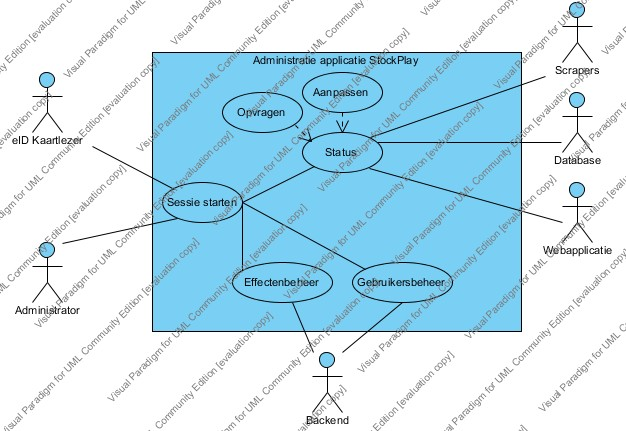
\includegraphics[width=0.5\textwidth]{images/analyse/ucd_desktop}
	\caption{Use-case diagram van de desktopapplicatie.}
\end{figure}

\subsubsection{Inloggen van gebruiker}
\begin{compact}
\paragraph{Beschrijving} Een gebruiker logt in op de desktopapplicatie via zijn e-ID.
\paragraph{Doel} De administrator is ingelogd op de desktopapplicatie en kan het spel nu beheren.
\paragraph{Triggers}De gebruiker opent de dekstopapplicatie.
\paragraph{Prioriteit}Gemiddeld
\paragraph{Complexiteit}Gemiddeld
\paragraph{Primaire actoren}Gebruiker, e-ID kaartlezer
\paragraph{Secundaire actoren}Back-end, databank
\paragraph{Successcenario}
\begin{enumerate_compact}
 \item De gebruiker krijgt een inlogscherm te zien.
 \item De applicatie vraagt de gebruiker om zijn identiteitskaart in de e-ID lezer te plaatsen en wacht tot dit voltooid is.
 \item De gebruiker plaatst zijn identiteitskaart in de e-ID lezer.
 \item De gebruiker krijgt een voortgangsbalk te zien.
 \item De applicatie leest de nodige gegevens van de identiteitskaart uit.
 \item Er wordt een aanvraag via XML-RPC gestuurd naar de backend om de gegevens te valideren.
 \item De backend raadpleegt de databank om de lijst van administrators op te halen.
 \item Na controle van de gegevens stuurt de backend een antwoord via XML-RPC naar de desktopapplicatie.
 \item De gebruiker is nu ingelogd en krijgt de statuspagina van de desktopappliactie te zien.
\end{enumerate_compact}
\paragraph{Alternatieve Scenario's}
\begin{enumerate_compact}
	\item[6.] Als een server niet beschikbaar is wordt een foutboodschap getoond.
	\item[8.] Indien de gebruiker niet geregistreerd staat als een administrator wordt een foutmelding getoond en komt hij terug terecht bij stap 2.
\end{enumerate_compact}
\end{compact}

\subsubsection{Status van servers bekijken}
\begin{compact}
\paragraph{Beschrijving} De administrator kan de onlinestatus van de verschillende servers bekijken op de statuspagina. De administrator kan de servers hier ook beheren.
\paragraph{Doel} De applicatie toont een paneel met daarin de status van de verschillende servers.
\paragraph{Triggers}De administrator moet ingelogd zijn en het statusmenu openen.
\paragraph{Prioriteit}Gemiddeld
\paragraph{Complexiteit}Laag
\paragraph{Primaire actoren}Administrator
\paragraph{Secundaire actoren}Back-end, databank
\paragraph{Successcenario}
\begin{enumerate_compact}
 \item De administrator opent het statusmenu.
 \item De desktopapplicatie vraagt de backend om de status van de verschillende servers te controleren.
 \item De applicatie toont een paneel met de status van de servers samen met mogelijke acties die de administrator kan ondernemen.
 \item In het menu worden snelkoppelingen naar uitgebreidere statuspagina's getoond.
\end{enumerate_compact}
\paragraph{Alternatieve Scenario's}
\begin{enumerate_compact}
	\item[2.] Als de backend niet antwoord wordt deze als offline beschouwd en krijgen de andere servers als status ``onbekend''.
	\item[4.] Indien de servers niet bereikbaar zijn, zijn deze koppelingen uitgegrijsd.
\end{enumerate_compact}
\end{compact}

\subsubsection{Gebruikersgegevens wijzigen}
\begin{compact}
\paragraph{Beschrijving} Een administrator kan gegevens van een gebruiker wijzigen via de desktopapplicatie.
\paragraph{Doel} De gegevens van de gespecificeerde gebruiker aanpassen in de databank.
\paragraph{Triggers}De administrator moet ingelogd zijn en het gebruikersbeheermenu openen.
\paragraph{Prioriteit}Hoog
\paragraph{Complexiteit}Gemiddeld
\paragraph{Primaire actoren}Administrator
\paragraph{Secundaire actoren}Back-end, databank
\paragraph{Successcenario}
\begin{enumerate_compact}
 \item De administrator opent het gebruikersbeheermenu.
 \item De applicatie vraagt een lijst van recent geregistreerde gebruikers op bij de back-end en ontvangt deze via XML-RPC. Deze lijst wordt getoond aan de gebruiker in de vorm van een tabel.
 \item De administrator past filters toe om de getoonde lijst te beperken tot de gewenste gebruikers.
 \item Alle gebruikers die aan de filter voldoen worden opgehaald uit de databank en de backend stuurt deze terug via XML-RPC.
 \item De administrator kiest een gebruiker uit de tabel en voert de actie ``Gebruiker bewerken'' uit.
 \item Er wordt een modaal venster getoond met daarin alle beschikbare gegevens van de gebruiker. Niet aanpasbare gegevens worden uitgegrijsd.
 \item De administrator brengt de gewenste wijzigen aan en kiest OK.
 \item De nieuwe gegevens worden doorgestuurd naar de backend.
 \item De backend voert de wijzigingen door in de databank.
 \item De administrator komt terug terecht in de tabel gebruikers.
\end{enumerate_compact}
\paragraph{Alternatieve Scenario's}
\begin{enumerate_compact}
	\item[2/3.] Als de servers niet bereikbaar zijn wordt een gepaste foutboodschap getoond.
	\item[9.] Indien er een fout optreedt bij het aanpassen van de gegevens in de databank wordt hier een melding van getoond en krijgt de administrator de kans om de ongeldige gegevens aan te passen.
\end{enumerate_compact}
\end{compact}

\subsubsection{Effect schorsen of verbergen}
\begin{compact}
\paragraph{Beschrijving} Als er problemen zijn met een bepaald effect kan een administrator deze schorsen om het verhandelen ervan onmogelijk te maken. Eventueel kan het effect ook onzichtbaar gemaakt worden.
\paragraph{Doel} Het effect is nu niet meer verhandelbaar in het spel, of is onzichtbaar gemaakt
\paragraph{Triggers}De administrator is ingelogd en bevindt zich in het effectenbeheermenu
\paragraph{Prioriteit}Hoog
\paragraph{Complexiteit}Laag
\paragraph{Primaire actoren}Administrator
\paragraph{Secundaire actoren}Back-end, databank
\paragraph{Successcenario}
\begin{enumerate_compact}
 \item De administrator opent het effectenbeheermenu.
 \item De applicatie toont alle beschikbare effecten in een tabel samen met hun belangrijkste gegevens.
 \item De administrator kan desgewenst een filter toepassen om de lijst te beperken.
 \item De administrator selecteert \'e\'en of meerdere effecten die hij wil aanpassen.
 \item De actie ``Effect(en) verbergen'' of ``Effect(en) schorsen'' wordt gekozen.
 \item De veranderingen worden doorgestuurd naar de backend en deze past de databank aan.
\end{enumerate_compact}
\paragraph{Alternatieve Scenario's}
\begin{enumerate_compact}
	\item[2.] Als de servers niet bereikbaar zijn wordt een gepaste foutboodschap getoond.
\end{enumerate_compact}
\end{compact}

\subsubsection{Gebruiker verbannen}
\begin{compact}
\paragraph{Beschrijving} Een administrator kan een gebruiker voor een bepaalde tijdsduur uit het spel verbannen.
\paragraph{Doel} De verbannen gebruiker kan niet meer inloggen gedurende de opgegeven tijdsduur.
\paragraph{Triggers}De administrator is ingelogd en opent het gebruikersbeheermenu
\paragraph{Prioriteit}Hoog
\paragraph{Complexiteit}Laag
\paragraph{Primaire actoren}Administrator
\paragraph{Secundaire actoren}Back-end, databank
\paragraph{Successcenario}
\begin{enumerate_compact}
 \item De administrator opent het gebruikersbeheermenu.
 \item De applicatie krijgt een beperkte lijst van gebruikers die het ontvangt vanuit de back-end.
 \item De administrator past filters toe om de getoonde lijst te beperken tot de gewenste gebruikers.
 \item Alle gebruikers die aan de filter voldoen worden opgehaald uit de databank en de backend stuurt deze terug via XML-RPC.
 \item De administrator selecteert de gewenste gebruikers en kiest voor ``Gebruiker deactiveren''.
 \item Er wordt een venster getoond met daarin de mogelijkheid om een tijdsduur in te geven of een checkbox die aangeeft dat deze gebruiker permanent moet verbannen worden.
 \item De wijzigingen worden gestuurd naar de backend en deze past de gebruikers aan in de databank.
 \item De administrator krijgt opnieuw het gebruikersoverzicht te zien.
\end{enumerate_compact}
\paragraph{Alternatieve Scenario's}
\begin{enumerate_compact}
	\item[2/4.] Een foutmelding wordt getoond als de backend niet bereikbaar is.
\end{enumerate_compact}
\end{compact}

\subsubsection{Schorsen van een effect}
\begin{compact}
\paragraph{Beschrijving} Een effect dat geschorst is op de beurs kan niet meer verhandeld worden. Dus het kan gekocht noch verkocht worden.
\begin{itemize_compact}
	\item De scraper haalt de JSON-feed op van de website en verwerkt hem
  \item Voor elke opgehaalde koers wordt een XML-RPC-aanroep naar de backend gestuurd met alle gegevens uit de opgehaalde gegevens
  \item De order-verwerking wordt gestart
  \item In de JSON-feed zit ook een timeout-veld. De scraper wacht met de volgende ophaling tot de opgelegde timeout verstreken is
\end{itemize_compact}
\paragraph{Precondities} De administrator 
\paragraph{Postcondities} De effect is geschorst
\paragraph{Prioriteit}Laag
\paragraph{Complexiteit}Laag
\end{compact}


\section{Backend}

\subsection{Uitwerking use cases}

\subsubsection{Scrapen van beurskoersen}
\begin{compact}
\paragraph{Beschrijving} De beurskoersen die in dit spel worden gebruikt worden constant live gescraped van enkele beurswebsites
\begin{itemize_compact}
	\item De scraper haalt de JSON-feed op van de website en verwerkt hem
  \item Voor elke opgehaalde koers wordt een XML-RPC-aanroep naar de backend gestuurd met alle gegevens uit de opgehaalde gegevens
  \item De order-verwerking wordt gestart
  \item In de JSON-feed zit ook een timeout-veld. De scraper wacht met de volgende ophaling tot de opgelegde timeout verstreken is
\end{itemize_compact}
\paragraph{Precondities} De beurs is open
\paragraph{Postcondities} De huidige koersen zijn in de database opgeslagen
\paragraph{Prioriteit}Hoog
\paragraph{Complexiteit}Hoog
\end{compact}

\subsubsection{Omzetten van orders naar transacties}
\begin{compact}
\paragraph{Beschrijving} Als een gebruiker een aandeel wil kopen of verkopen moet hij daar een order voor aanmaken. De effectieve uitvoering van een order gebeurt dan door de beurs zelf. In dit spel gebeurt dit door de backend. Deze controleert elke minuut of de condities voor het order voldaan zijn, en voert deze uit indien ze in orde zijn.
\begin{itemize_compact}
	\item Alle orders worden opgevraagd
  \item Voor elke order gebeuren dan de volgende stappen:
	\begin{itemize_compact}
		\item De condities opgegeven in het order worden gecontroleerd (heeft de koers de opgegeven waarde bereikt, is het effect niet geschorst, etc)
		\item De order wordt uit het systeem verwijderd
		\item De transactie wordt in het systeem ingegeven
	\end{itemize_compact}
\end{itemize_compact}
\paragraph{Precondities} De beurs is open 
\paragraph{Postcondities} De orders waarvan de condities voldaan zijn, werden omgezet naar effectieve transactie.
\paragraph{Prioriteit}Matig
\paragraph{Complexiteit}Matig
\end{compact}


%
% Functieanalyse
%

\chapter{Functieanalyse}

\todo{Hier komt een beschrijving van de omgeving waarin het systeem moet werken}
